
%% bare_conf.tex
%% V1.4a
%% 2014/09/17
%% by Michael Shell
%% See:
%% http://www.michaelshell.org/
%% for current contact information.
%%
%% This is a skeleton file demonstrating the use of IEEEtran.cls
%% (requires IEEEtran.cls version 1.8a or later) with an IEEE
%% conference paper.
%%
%% Support sites:
%% http://www.michaelshell.org/tex/ieeetran/
%% http://www.ctan.org/tex-archive/macros/latex/contrib/IEEEtran/
%% and
%% http://www.ieee.org/

%%*************************************************************************
%% Legal Notice:
%% This code is offered as-is without any warranty either expressed or
%% implied; without even the implied warranty of MERCHANTABILITY or
%% FITNESS FOR A PARTICULAR PURPOSE! 
%% User assumes all risk.
%% In no event shall IEEE or any contributor to this code be liable for
%% any damages or losses, including, but not limited to, incidental,
%% consequential, or any other damages, resulting from the use or misuse
%% of any information contained here.
%%
%% All comments are the opinions of their respective authors and are not
%% necessarily endorsed by the IEEE.
%%
%% This work is distributed under the LaTeX Project Public License (LPPL)
%% ( http://www.latex-project.org/ ) version 1.3, and may be freely used,
%% distributed and modified. A copy of the LPPL, version 1.3, is included
%% in the base LaTeX documentation of all distributions of LaTeX released
%% 2003/12/01 or later.
%% Retain all contribution notices and credits.
%% ** Modified files should be clearly indicated as such, including  **
%% ** renaming them and changing author support contact information. **
%%
%% File list of work: IEEEtran.cls, IEEEtran_HOWTO.pdf, bare_adv.tex,
%%                    bare_conf.tex, bare_jrnl.tex, bare_conf_compsoc.tex,
%%                    bare_jrnl_compsoc.tex, bare_jrnl_transmag.tex
%%*************************************************************************


% *** Authors should verify (and, if needed, correct) their LaTeX system  ***
% *** with the testflow diagnostic prior to trusting their LaTeX platform ***
% *** with production work. IEEE's font choices and paper sizes can       ***
% *** trigger bugs that do not appear when using other class files.       ***                          ***
% The testflow support page is at:
% http://www.michaelshell.org/tex/testflow/



\documentclass[conference]{acm_sen_article}
% Some Computer Society conferences also require the compsoc mode option,
% but others use the standard conference format.
%
% If IEEEtran.cls has not been installed into the LaTeX system files,
% manually specify the path to it like:
% \documentclass[conference]{../sty/IEEEtran}

\setlength{\paperheight}{11in}
\setlength{\paperwidth}{8.5in}
\usepackage[pass]{geometry}
\usepackage{verbatim}
\usepackage{url}
\usepackage{listings}
\usepackage{color}
\usepackage{multicol}
\usepackage{paralist}
\usepackage{comment}
\usepackage{hyperref}

\newcommand{\figref}[1]{Figure~\ref{#1}}
\newcommand{\tableref}[1]{Table~\ref{#1}}
\newcommand{\secref}[1]{Section~\ref{#1}}

\definecolor{dkgreen}{rgb}{0,0.6,0}
\definecolor{gray}{rgb}{0.5,0.5,0.5}
\definecolor{mauve}{rgb}{0.58,0,0.82}

\lstset{frame=tb,
  language=Java,
  aboveskip=3mm,
  belowskip=3mm,
  showstringspaces=false,
  columns=flexible,
  basicstyle={\small\ttfamily},
  numbers=none,
  numberstyle=\tiny\color{gray},
  keywordstyle=\color{blue},
  commentstyle=\color{dkgreen},
  stringstyle=\color{mauve},
  breaklines=true,
  breakatwhitespace=true
  tabsize=3
}

% Some very useful LaTeX packages include:
% (uncomment the ones you want to load)


% *** MISC UTILITY PACKAGES ***
%
%\usepackage{ifpdf}
% Heiko Oberdiek's ifpdf.sty is very useful if you need conditional
% compilation based on whether the output is pdf or dvi.
% usage:
% \ifpdf
%   % pdf code
% \else
%   % dvi code
% \fi
% The latest version of ifpdf.sty can be obtained from:
% http://www.ctan.org/tex-archive/macros/latex/contrib/oberdiek/
% Also, note that IEEEtran.cls V1.7 and later provides a builtin
% \ifCLASSINFOpdf conditional that works the same way.
% When switching from latex to pdflatex and vice-versa, the compiler may
% have to be run twice to clear warning/error messages.






% *** CITATION PACKAGES ***
%
%\usepackage{cite}
% cite.sty was written by Donald Arseneau
% V1.6 and later of IEEEtran pre-defines the format of the cite.sty package
% \cite{} output to follow that of IEEE. Loading the cite package will
% result in citation numbers being automatically sorted and properly
% "compressed/ranged". e.g., [1], [9], [2], [7], [5], [6] without using
% cite.sty will become [1], [2], [5]--[7], [9] using cite.sty. cite.sty's
% \cite will automatically add leading space, if needed. Use cite.sty's
% noadjust option (cite.sty V3.8 and later) if you want to turn this off
% such as if a citation ever needs to be enclosed in parenthesis.
% cite.sty is already installed on most LaTeX systems. Be sure and use
% version 5.0 (2009-03-20) and later if using hyperref.sty.
% The latest version can be obtained at:
% http://www.ctan.org/tex-archive/macros/latex/contrib/cite/
% The documentation is contained in the cite.sty file itself.






% *** GRAPHICS RELATED PACKAGES ***
%

\usepackage{graphicx}

%\ifCLASSINFOpdf
 % \usepackage[pdftex]{graphicx}
  % declare the path(s) where your graphic files are
  % \graphicspath{{../pdf/}{../jpeg/}}
  % and their extensions so you won't have to specify these with
  % every instance of \includegraphics
  % \DeclareGraphicsExtensions{.pdf,.jpeg,.png}
%\else
  % or other class option (dvipsone, dvipdf, if not using dvips). graphicx
  % will default to the driver specified in the system graphics.cfg if no
  % driver is specified.
  % \usepackage[dvips]{graphicx}
  % declare the path(s) where your graphic files are
  % \graphicspath{{../eps/}}
  % and their extensions so you won't have to specify these with
  % every instance of \includegraphics
  % \DeclareGraphicsExtensions{.eps}
%\fi
% graphicx was written by David Carlisle and Sebastian Rahtz. It is
% required if you want graphics, photos, etc. graphicx.sty is already
% installed on most LaTeX systems. The latest version and documentation
% can be obtained at: 
% http://www.ctan.org/tex-archive/macros/latex/required/graphics/
% Another good source of documentation is "Using Imported Graphics in
% LaTeX2e" by Keith Reckdahl which can be found at:
% http://www.ctan.org/tex-archive/info/epslatex/
%
% latex, and pdflatex in dvi mode, support graphics in encapsulated
% postscript (.eps) format. pdflatex in pdf mode supports graphics
% in .pdf, .jpeg, .png and .mps (metapost) formats. Users should ensure
% that all non-photo figures use a vector format (.eps, .pdf, .mps) and
% not a bitmapped formats (.jpeg, .png). IEEE frowns on bitmapped formats
% which can result in "jaggedy"/blurry rendering of lines and letters as
% well as large increases in file sizes.
%
% You can find documentation about the pdfTeX application at:
% http://www.tug.org/applications/pdftex





% *** MATH PACKAGES ***
%
%\usepackage[cmex10]{amsmath}
% A popular package from the American Mathematical Society that provides
% many useful and powerful commands for dealing with mathematics. If using
% it, be sure to load this package with the cmex10 option to ensure that
% only type 1 fonts will utilized at all point sizes. Without this option,
% it is possible that some math symbols, particularly those within
% footnotes, will be rendered in bitmap form which will result in a
% document that can not be IEEE Xplore compliant!
%
% Also, note that the amsmath package sets \interdisplaylinepenalty to 10000
% thus preventing page breaks from occurring within multiline equations. Use:
%\interdisplaylinepenalty=2500
% after loading amsmath to restore such page breaks as IEEEtran.cls normally
% does. amsmath.sty is already installed on most LaTeX systems. The latest
% version and documentation can be obtained at:
% http://www.ctan.org/tex-archive/macros/latex/required/amslatex/math/






% *** SPECIALIZED LIST PACKAGES ***
%
%\usepackage{algorithmic}
% algorithmic.sty was written by Peter Williams and Rogerio Brito.
% This package provides an algorithmic environment fo describing algorithms.
% You can use the algorithmic environment in-text or within a figure
% environment to provide for a floating algorithm. Do NOT use the algorithm
% floating environment provided by algorithm.sty (by the same authors) or
% algorithm2e.sty (by Christophe Fiorio) as IEEE does not use dedicated
% algorithm float types and packages that provide these will not provide
% correct IEEE style captions. The latest version and documentation of
% algorithmic.sty can be obtained at:
% http://www.ctan.org/tex-archive/macros/latex/contrib/algorithms/
% There is also a support site at:
% http://algorithms.berlios.de/index.html
% Also of interest may be the (relatively newer and more customizable)
% algorithmicx.sty package by Szasz Janos:
% http://www.ctan.org/tex-archive/macros/latex/contrib/algorithmicx/




% *** ALIGNMENT PACKAGES ***
%
%\usepackage{array}
% Frank Mittelbach's and David Carlisle's array.sty patches and improves
% the standard LaTeX2e array and tabular environments to provide better
% appearance and additional user controls. As the default LaTeX2e table
% generation code is lacking to the point of almost being broken with
% respect to the quality of the end results, all users are strongly
% advised to use an enhanced (at the very least that provided by array.sty)
% set of table tools. array.sty is already installed on most systems. The
% latest version and documentation can be obtained at:
% http://www.ctan.org/tex-archive/macros/latex/required/tools/


% IEEEtran contains the IEEEeqnarray family of commands that can be used to
% generate multiline equations as well as matrices, tables, etc., of high
% quality.




% *** SUBFIGURE PACKAGES ***
%\ifCLASSOPTIONcompsoc
%  \usepackage[caption=false,font=normalsize,labelfont=sf,textfont=sf]{subfig}
%\else
%  \usepackage[caption=false,font=footnotesize]{subfig}
%\fi
% subfig.sty, written by Steven Douglas Cochran, is the modern replacement
% for subfigure.sty, the latter of which is no longer maintained and is
% incompatible with some LaTeX packages including fixltx2e. However,
% subfig.sty requires and automatically loads Axel Sommerfeldt's caption.sty
% which will override IEEEtran.cls' handling of captions and this will result
% in non-IEEE style figure/table captions. To prevent this problem, be sure
% and invoke subfig.sty's "caption=false" package option (available since
% subfig.sty version 1.3, 2005/06/28) as this is will preserve IEEEtran.cls
% handling of captions.
% Note that the Computer Society format requires a larger sans serif font
% than the serif footnote size font used in traditional IEEE formatting
% and thus the need to invoke different subfig.sty package options depending
% on whether compsoc mode has been enabled.
%
% The latest version and documentation of subfig.sty can be obtained at:
% http://www.ctan.org/tex-archive/macros/latex/contrib/subfig/




% *** FLOAT PACKAGES ***
%
%\usepackage{fixltx2e}
% fixltx2e, the successor to the earlier fix2col.sty, was written by
% Frank Mittelbach and David Carlisle. This package corrects a few problems
% in the LaTeX2e kernel, the most notable of which is that in current
% LaTeX2e releases, the ordering of single and double column floats is not
% guaranteed to be preserved. Thus, an unpatched LaTeX2e can allow a
% single column figure to be placed prior to an earlier double column
% figure. The latest version and documentation can be found at:
% http://www.ctan.org/tex-archive/macros/latex/base/


%\usepackage{stfloats}
% stfloats.sty was written by Sigitas Tolusis. This package gives LaTeX2e
% the ability to do double column floats at the bottom of the page as well
% as the top. (e.g., "\begin{figure*}[!b]" is not normally possible in
% LaTeX2e). It also provides a command:
%\fnbelowfloat
% to enable the placement of footnotes below bottom floats (the standard
% LaTeX2e kernel puts them above bottom floats). This is an invasive package
% which rewrites many portions of the LaTeX2e float routines. It may not work
% with other packages that modify the LaTeX2e float routines. The latest
% version and documentation can be obtained at:
% http://www.ctan.org/tex-archive/macros/latex/contrib/sttools/
% Do not use the stfloats baselinefloat ability as IEEE does not allow
% \baselineskip to stretch. Authors submitting work to the IEEE should note
% that IEEE rarely uses double column equations and that authors should try
% to avoid such use. Do not be tempted to use the cuted.sty or midfloat.sty
% packages (also by Sigitas Tolusis) as IEEE does not format its papers in
% such ways.
% Do not attempt to use stfloats with fixltx2e as they are incompatible.
% Instead, use Morten Hogholm'a dblfloatfix which combines the features
% of both fixltx2e and stfloats:
%
% \usepackage{dblfloatfix}
% The latest version can be found at:
% http://www.ctan.org/tex-archive/macros/latex/contrib/dblfloatfix/




% *** PDF, URL AND HYPERLINK PACKAGES ***
%
%\usepackage{url}
% url.sty was written by Donald Arseneau. It provides better support for
% handling and breaking URLs. url.sty is already installed on most LaTeX
% systems. The latest version and documentation can be obtained at:
% http://www.ctan.org/tex-archive/macros/latex/contrib/url/
% Basically, \url{my_url_here}.




% *** Do not adjust lengths that control margins, column widths, etc. ***
% *** Do not use packages that alter fonts (such as pslatex).         ***
% There should be no need to do such things with IEEEtran.cls V1.6 and later.
% (Unless specifically asked to do so by the journal or conference you plan
% to submit to, of course. )


% correct bad hyphenation here
\hyphenation{op-tical net-works semi-conduc-tor}


\begin{document}
%
% paper title
% Titles are generally capitalized except for words such as a, an, and, as,
% at, but, by, for, in, nor, of, on, or, the, to and up, which are usually
% not capitalized unless they are the first or last word of the title.
% Linebreaks \\ can be used within to get better formatting as desired.
% Do not put math or special symbols in the title.
\title{Verification of Habanero Java Programs using Computation Graphs}


% author names and affiliations
% use a multiple column layout for up to three different
% affiliations
%\author{\IEEEauthorblockN{Radha Nakade}
%\IEEEauthorblockA{ Brigham Young University\\
%Provo, Utah\\
%Email: radha.nakade@gmail.com}
%\and
%\IEEEauthorblockN{Eric Mercer}
%\IEEEauthorblockA{Brigham Young University\\
%Provo, Utah\\
%Email: egm@cs.byu.edu}}
\numberofauthors{2}

\author{
\alignauthor
Radha Nakade\\
       \affaddr{Brigham Young University}\\
       \affaddr{Provo, Utah}\\
       \email{radha.nakade@gmail.com}    
\alignauthor
Eric Mercer \\
       \affaddr{Brigham Young University}\\
       \affaddr{Provo, Utah}\\
       \email{egm@cs.byu.edu} }


% make the title area
\maketitle

% As a general rule, do not put math, special symbols or citations
% in the abstract
\begin{abstract}
The Habanero Java (HJ) programming model is designed to provide several correctness guarantees such as deadlock freedom and determinism in the absence of data races. Model checking tools like Java Pathfinder (JPF) can be used to detect data races in HJ programs. But, as the program size increases, data race detection becomes expensive because of the state space explosion. We present a new method of data race detection in HJ programs with the help of computation graphs. A computation graph represents the execution of a program in the form of a directed acyclic graph. For structurally deterministic programs, analyzing the graph on a single schedule is enough for data race detection.
\end{abstract}

% no keywords




% For peer review papers, you can put extra information on the cover
% page as needed:
% \ifCLASSOPTIONpeerreview
% \begin{center} \bfseries EDICS Category: 3-BBND \end{center}
% \fi
%
% For peerreview papers, this IEEEtran command inserts a page break and
% creates the second title. It will be ignored for other modes.
%\IEEEpeerreviewmaketitle



%\section{Introduction}
% no \IEEEPARstart

\section{Introduction}
The increasing use of multicore processors is motivating the use of parallel programming. However, it is very difficult to write concurrent programs that are free from bugs. When programs execute different instructions simultaneously, different thread schedules and memory access patterns are observed that give rise to various issues such as data-races, deadlocks etc. To make writing concurrent programs easier, Rice University developed Habanero Java Programming model \cite{Cave:2011:HNA:2093157.2093165}. It provides safety guarantees such as deadlock freedom, deterministic output and serialization for subsets of constructs provided in the programming model. These guarantees hold only in the absence of data-races. The Habanero Java library (HJ-Lib) \cite{hj-lib} is a Java 8 library implementation of the Habanero Java programming model.

VR-lib \cite{Anderson:2015:JVH:2693208.2693245}, a verification runtime for HJ programs was built at Brigham Young University. VR-lib facilitates the verification of HJ programs using JPF. VR-lib can be used along with JPF to build computation graphs of HJ programs. A Computation Graph (CG) is an acyclic directed graph that consists of a set of nodes, where each node represents a step consisting of some sequential execution of the program and a set of edges that represent the ordering of the steps. A CG stores the memory locations accessed and updated by each of the operators. It also correctly reflects the control flow structure of the program.

The CGRaceDetector listener presented in this work monitors the various object creations and destructions, instruction executions etc to build a computation graph for the HJ program under a single schedule. It later analyzes this graph to verify any data access violations to report data races. For structurally deterministic programs, verifying the HJ program under a single schedule is enough to detect data races.

Section 2 of this paper presents an overview of the Habanero Java programming model and gives a brief description for the various parallel constructs of HJ language. Section 3 describes the computation graphs and its various elements. It also gives the implementation details of computation graph builder and analyzer for HJ programs created with the help of JPF. Section 4 describes the preliminary results of the CGRaceDetector on some HJ micro-benchmarks. Section 5 concludes and outlines the ways to  extend this work.

\begin{figure}[t]
\centering
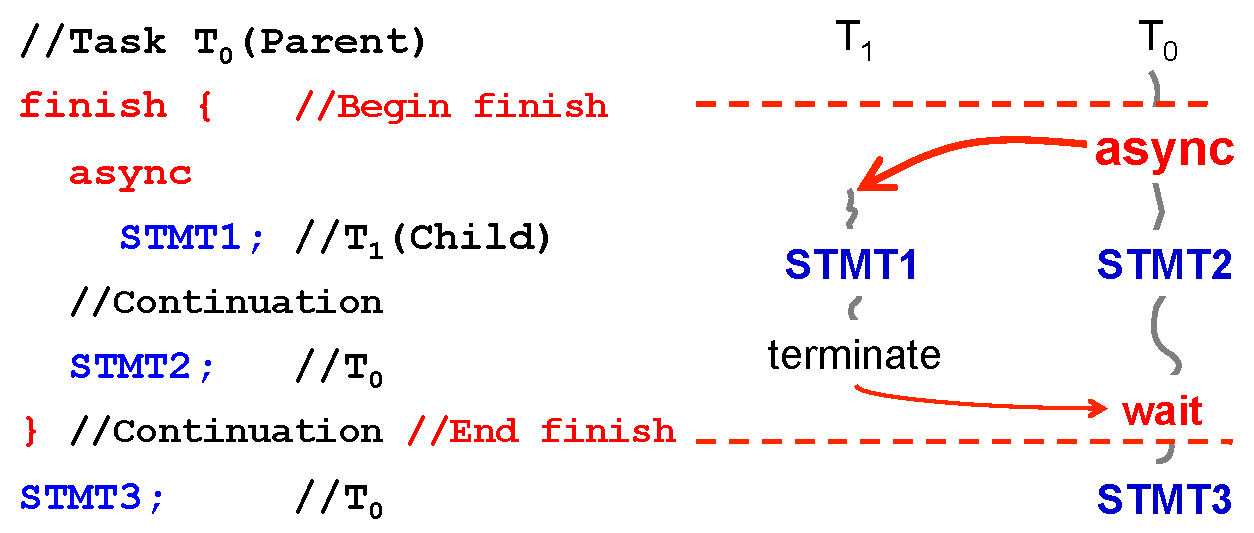
\includegraphics[width=3.25in]{../figs/async-finish}
\caption{An example with {\tt async} and {\tt finish}.}
\label{fig:async-finish}
\end{figure}


\section{Habanero Programming Model}

The Habanero programming model is built around a task-parallel view of
concurrency \cite{Cave:2011:HNA:2093157.2093165}. \figref{fig:async-finish} illustrates Habanero in its
simplest form \cite{Cave:2011:HNA:2093157.2093165}.

The \texttt{async}-construct is a mechanism for
creating a new asynchronous task: {\tt async}
$\langle${\em stmt}$\rangle$ causes the calling task (i.e., the
parent) to create a new child task to execute {\em
  $\langle$stmt$\rangle$} (logically) in parallel with the parent
task. {\em $\langle$stmt$\rangle$} can read or write any data in the
heap and can read (but not write) any local variable belonging to the
parent task's lexical scope. The task created by any
\texttt{async}-construct is scheduled at the point it is declared in
the program.

The \texttt{finish}-construct is a generalized join operation for
collective synchronization: {\tt finish} $\langle${\em
  stmt}$\rangle$ causes the parent task to execute {\em
  $\langle$stmt$\rangle$} and then wait until all tasks created within
{\em $\langle$stmt$\rangle$} have completed, including transitively
created tasks.  Each dynamic instance of a task has a unique {\em
  immediately-enclosing-finish} (IEF) during program execution. That IEF is the
innermost {\tt finish}-construct containing the task.  There is an implicit {\tt
  finish}-construct surrounding the entry point of the program so the program only terminates after
all tasks have completed.

A computation graph illustrating the semantics of the \texttt{async}
and \texttt{finish} constructs is on the right side of
\figref{fig:async-finish}. In the graph, task $T_0$ enters the
\texttt{finish}-construct, creates task $T_1$ at the
\texttt{async}-construct, and then continues on to
\texttt{STMT2}. After \texttt{STMT2}, $T_0$ waits for $T_1$ to
complete before moving on to \texttt{STMT3}. Note that \texttt{STMT1}
and \texttt{STMT2} are not ordered by the semantics and represent
parallel execution.

Habanero supports more advanced forms of tasking beyond creation and
collective synchronization. The \texttt{isolated}-construct, {\tt isolated}~$\langle${\it
  stmt1}$\rangle$, ensures that $\langle${\it stmt1}$\rangle$ is
evaluated in mutual exclusion with all other {\tt
  isolated}-constructs.  There are two subtle nuances in the Habanero
model for the \texttt{isolated}-construct:
\begin{compactenum}
\item The construct ensures mutual exclusion between \texttt{isolated}-constructs and not mutual exclusion on a particular memory location. Mutual exclusion on a particular memory location is implemented by wrapping operations on that memory location in \texttt{isolated}-constructs. 
\item Any Habanero implementation may relax mutual-exclusion between
  \texttt{isolated}-constructs as long as the constructs do not
  interfere with one another. Interference in this context means that
  multiple \texttt{isolated}-constructs access a common memory
  location and at least one of those accesses is a write.
\end{compactenum}

The \texttt{future}-construct lets tasks
return values to other tasks: \textbf{future} {\em f} $=$ \textbf{async}
  $\langle${\em expr}$\rangle$ creates a new child task to evaluate $\langle${\em expr}$\rangle$.  The local
variable {\em f} contains a \emph{future handle} to the newly created
task that can be used to obtain the value produced by $\langle${\em expr}$\rangle$. The blocking operation {\em f.get()} returns that value when the
child task completes.

The most complex construct in the Habanero model is the
\textit{phaser} \cite{Shirako:2008:PUD:1375527.1375568}. A phaser is a form of a barrier that provides
point-to-point fine-grain synchronization between tasks to coordinate
their movement through \emph{phases} of computation. Like barriers, phasers order execution of
portions of the program into phases and restrict tasks from
entering the next phase until the current phase is complete. Unlike
barriers though, phasers allow tasks to specify point-to-point relationships on
multiple phasers, and tasks can dynamically join or leave the phaser.

Tasks register with an instance of a phaser, and on registration,
declare the mode that control how that task
synchronizes relative to other tasks registered on the same
barrier. Synchronization takes place with the \texttt{next}-construct
which may block depending on the state of the phaser, and on how the task is registered with the phaser.
\begin{compactitem}
\item \texttt{SIG}: signal registration means all tasks that have designated themselves as signalers must signal the phaser
in order for the phase to advance.  The \texttt{next}-construct for a signal-only task signals the phaser and immediately advances to the next phase.  The phaser remembers each phase completed by any task.
\item \texttt{SIG\_WAIT}: \emph{signal-wait} registration means the task signals the phaser and then waits for other tasks to complete the phase. This registration mode functions like a traditional barrier. The \texttt{next}-construct for a signal-wait task reports phase completion and then blocks for the other signalers to complete the phase too.
\item \texttt{WAIT}: \emph{wait} registration means that the task blocks at the \texttt{next}-construct until the phase advances. 
\end{compactitem}
Phasers may also be bounded to specify slack in the number of phases that may separate
waiters and signalers so signalers can work ahead of waiters
up to a bound.\footnote{Omitted in this presentation of phasers is the ability of a single task to execute constructs after the end of one phase and before the start of the next phase.}

Habanero includes several other constructs such as
\texttt{foreach}-constructs, \texttt{forall}-constructs, \emph{data
  driven futures}, \emph{actors}, etc. most of which are syntactic
sugar for the presented constructs.


\section{Computation graphs}
The execution of a task-parallel program can be represented in the form of a computation graph. A computation graph of a program is a directed acyclic graph (DAG) structure that represents the sequence of execution of tasks in the parallel program. A computation graph can be represented as G = $\langle$V, E$\rangle$ where
\begin{itemize}
\item V is a set of nodes such that  each node represents a step consisting of an arbitrary sequential computation and
\item E is a set of directed edges that represent ordering constraints. The various types of edges in a computation graph are:
%\begin{enumerate}
\begin{itemize}
 \item \textbf{Spawn edges:} They connect steps in parent tasks to steps in child async tasks. When an async is created, a spawn edge is inserted between the step that ends with the async in the parent task and the step that starts the async body in the new child task.
\item \textbf{Join edges:} They connect steps in descendant tasks to steps in the tasks containing their Immediately Enclosing Finish (IEF) instances. When an async terminates, a join edge is inserted from the last step in the async to the step that follows the IEF operation in the task containing the IEF operation.
\item \textbf{Continue edges:} They capture sequencing of steps within a task - all steps within the same task are connected by a chain of continue edges.
\item \textbf{Serialization edges:} They connect two isolated nodes S and S' where nodes S and S' are interfering. Two isolated nodes do not interfere only if they have a total ordering in the CG.
% \end{enumerate} 
\end{itemize}
\end{itemize}

Computation graphs provide a visual feedback of the execution of HJ programs. Computation graphs can be used not just to find concurrency bugs in parallel  programs but also to optimize the code. In this work, we concentrate only on data race detection in HJ programs with the help of computation graphs.

\textbf{Implementation Details:}
The CG builder is implemented using JPF. It uses the VR-lib, specifically designed to run HJ programs using JPF. The HJ program is compiled using the VR and the class files are analyzed using JPF. JPF creates thread choice generators to systematically explore the state-space of the programs. We choose one set of thread interleavings to build a CG for that execution. JPF tracks references to all the variables in the program. It also computes the aliasing information during runtime. These memory references are stored in the CG. The CGs are stored in a DAG data structure. 

Data races can be detected in a CG when two parallel nodes in the graph access a memory location and at least one of the operations tries to modify it. A topological traversal of the graph gives the order of execution of the various tasks. All the nodes that occur between a pair of Finish-start and Finish-end nodes execute in parallel. The global memory accesses by these processes is checked and if conflicting memory-accesses are observed, then a data race is reported.
\section{Implementation and Results}
\label{sec:res}

The data race detection technique described in this paper has been implemented for Habanero Java. It uses the verification runtime specifically designed to test HJ programs \cite{anderson2014jpf}. This runtime makes use of JPF to schedule and run the programs. JPF is essentially a fully customizable Java virtual machine. JPF is modified by removing its default scheduling-factory that inserts choices on all thread actions and accesses to shared variables. Instead, a new scheduling factory based on Algorithm \ref{algo:isolated} is employed for scheduling. The computation graphs are stored in a directed acyclic graph \cite{jgrapht}. The computation graphs are exported in the dot file format for convenience and as a way to understand the structure of the program \cite{graphviz}.

The data-race detector is created by implementing the methods in the \textit{PropertyListenerAdapter} to create the computation graph. When the runtime passes an object of the type \textit{Task} to the \texttt{objectCreated} method, the \textsc{Post} rule is invoked that adds a new node to the computation graph. When the \textit{stop-finish} is executed, the \textsc{Await-next} rule is invoked that creates a node in the graph to synchronize the tasks in the finish block. The \texttt{executeInstruction} method is used to track memory locations that are accessed by various tasks by updating the node with the location accessed by the task during the execution of that instruction.

The results for this technique have been compared to two approaches implemented by JPF: \textit{Precise race detector} and \textit{Gradual permission regions} on benchmarks that cover a wide range of functionality in HJ. These two approaches are specifically chosen for comparison since the results generated by these approaches are sound for a given input just like the technique discussed in this paper. The results show a significant improvement in the time required for verification. 

The benchmarks used in this study make use of various HJ constructs for achieving task parallelism. They spawn a wide range of tasks with smaller programs having 3-15 tasks going all the way up to 525 tasks for larger programs. The experiments were run on a machine with an Intel Core i5 processor with 2.6GHz speed and 8GB of RAM.

\begin{table*}
\centering
\caption{Benchmarks of HJ programs: Computation graphs vs Permission Regions vs. PreciseRaceDetector}
\rowcolors{1}{light-gray}{white}
\label{tab:results}
\resizebox{\textwidth}{!}{
\begin{tabular}{|m{3.5cm}|c|c|c|c|c|c|c|c|c|c|c|}
\hiderowcolors
\hline
        &      &       & 
        \multicolumn{3}{c|}{\textbf{\textit{Computation graphs}}} & 
		 \multicolumn{3}{c|}{\textbf{\textit{Gradual permission regions}}} &
		\multicolumn{3}{c|}{\textbf{\textit{Precise race detector}}} \\ \hline
		
\textbf{Test ID }& \textbf{SLOC} & \textbf{Tasks} 
& \textbf{States}  & \textbf{Time}  & \textbf{Error Note }
& \textbf{States}  & \textbf{Time}  & \textbf{Error Note }
& \textbf{States}  & \textbf{Time}  & \textbf{Error Note }     \\ \hline

\showrowcolors

\textit{Primitive Array Race} & 39 & 3 
%& 5 & 00:00 & Race
& 5 & 00:00 & Race
& 5 & 00:00 & Race
& 220 & 00:00 & Race \\ \hline

\textit{Substring Search}  & 83 & 59 
%& 64 & 00:03 & Race
& 64 & 00:03 & Race
& 8 & 00:00 & Race 
& N/A & N/A & N/A \\ \hline

\textit{Reciprocal Array Sum} & 58 & 2
%& 12 & 0:00:16 & Race
& 4 & 00:08 & Race
& 32 & 00:06 & Race
& N/A & N/A & N/A \\ \hline

\textit{Primitive Array No Race} & 29 & 3 
%& 5 & 00:00 & No Race
& 5 & 00:00 & No Race
& 5 & 00:00 & No Race 
& 11,852 & 00:00 & No Race \\ \hline

\textit{Two Dim Arrays }& 30 & 11 
%& 15 & 00:01 & No Race
& 15 & 00:00 & No Race
& 15 & 00:00 & No Race 
& 597 & 00:00 & Race* \\ \hline

\textit{ForAll With Iterable} & 38 & 2
%& 9 & 00:00 & No Race
& 9 & 00:00 & No Race
& 9 & 00:00 & No Race 
& N/A & N/A & N/A \\ \hline

\textit{Integer Counter  Isolated} & 54 & 10
%& 24 & 00:01 & No Race
& 24 & 00:01 & No Race
& 1,013,102 & 05:53 & No Race 
& N/A & N/A & N/A \\ \hline

\textit{Pipeline With Futures} & 69 & 5
%& 34 & 0:00:00 & No Race
& 34 & 00:00 & No Race
& 34 & 00:00 & No Race 
& N/A & N/A & N/A \\ \hline

\textit{Binary Trees }& 80 & 525 
%& 632 & 0:00:05 & No Race
& 630 & 00:25 & No Race
& 632 & 00:03 & No Race 
& N/A & N/A & N/A \\ \hline

\textit{Prime Num Counter} & 51 & 25
%& 776 & 00:01 & No Race
& 776 & 00:01 & No Race
& 3,542,569 & 17:37 & No Race 
& N/A & N/A & N/A \\ \hline

\textit{Prime Num  Counter ForAll}  & 52 & 25
%& 30 & 0:00:02 & Race*
& 30 & 00:02 & No Race
& 18 & 00:01 & No Race
& N/A & N/A & N/A \\ \hline

\textit{Prime Num Counter ForAsync}  & 44 & 11 
%& 653 & 0:00:01 & No Race
& 653 & 00:01 & No Race
& 2,528,064 & 15:44 & No Race 
& N/A & N/A & N/A \\ \hline

\textit{Add}  & 67 & 3 
%& 11 & 0:00:01 & No Race 
& 11 & 00:01 & No Race 
& 62,374 & 00:33 & No Race
& 4930 & 00:03 & Race* \\ \hline

\textit{Scalar Multiply}  & 55 & 3 
%& 15 & 0:00:01 & No Race
& 15 & 00:01 & No Race
& 55,712 & 00:30 & No Race 
& 826 & 00:01 & Race* \\ \hline

\textit{Vector Add} & 50 & 3 
%& 5 & 0:00:01 & No Race
& 5 & 00:00 & No Race
& 17 & 00:00 & No Race 
& 46,394 & 00:19 & No Race \\ \hline

\textit{Clumped Access}  & 30 & 3 
%& 9 & 0:00:07 & No Race
& 5 & 00:03 & No Race
& 15 & 00:00 & No Race 
& N/A & N/A & N/A \\ \hline

\end{tabular}}
\vspace{-1em}
\end{table*}

\tableref{tab:results} presents the results of verification of the HJ benchmarks. The number of states explored by JPF and time required for verification by each method is compared. The tests are run for a maximum of an hour before they are terminated manually. If a test does not finish in the time bound or if it runs out of JVM memory, then it is marked as N/A in the table. The error note column shows the results of verification. The tests that produce erroneous results are marked with an asterisk ($\ast$). 

The \textit{Precise race detector} explores all potential executions of the program in a systematic way. Each execution is a sequence of transitions. Each transition takes the system from one state to another. Each transition consists of a sequence of byte-code instructions. JPF groups byte-code instructions such that an instruction that manipulates a shared variable is the first one of a transition. In every state that JPF visits, the \textit{precise race detector} checks all actions that can be performed next. If this collection of actions contains at least two conflicting accesses to a shared variable, then a data-race on the shared variable is reported. The \textit{precise race detector} inserts choices in the scheduler for all thread actions such as thread creation, synchronizations, locks etc. Therefore, it does not complete execution within the stipulated time or runs out of memory even on smaller programs because of the state space explosion. It also reports race for \textit{Two Dimensional Arrays}, \textit{Scalar multiply} and \textit{Vector Add} benchmarks where no data race actually exists in the program. This error is because in precise race detector, the access on an array object looks like a data race since it is not able to see the difference in the indexes.

\textit{Gradual permission regions} use program annotations to reduce the state space of the program \cite{mercer2015model}. Whenever a shared variable is accessed by multiple tasks in the program, the accesses have to be annotated to inform the data-race detector to create different schedules for these accesses. It is prone to human errors because of the need for manual annotation. If the program is annotated incorrectly, the results of data race detection analysis are no longer sound. \textit{gradual permission regions} works better than \textit{precise race detector}. Compared to \textit{computation graphs} in this paper though it falls behind quickly when there are several regions to annotate. A single execution is all that is needed for the \textit{computation graph analysis} while \textit{permission regions} have to enumerate an exponential number of schedules over the regions. The difference in performance is seen in the \textit{Add}, \textit{Scalar multiply} and \textit{Prime number counter} benchmarks. These benchmarks use shared variables that have to be enclosed within regions which results in a large state space for permission regions. The \textit{Prime number counter} benchmark also has isolated sections and therefore, the state space for \textit{computation graphs} is also large compared to other benchmarks.

We also evaluated our data race detector on some real world benchmarks. The \textit{Crypt-af} and \textit{Crypt-f} benchmarks are implementation of the IDEA encrytion algorithm and \textit{Series-af} and \textit{Series-f} are the Fourier coefficient analysis benchmarks adapted from the JGF suite \cite{bull2000benchmark} using \textbf{async-finish} and \textbf{future} constructs respectively. The \textit{strassen} benchmark is adapted from the  OpenMP version of the program in the Kastors suite \cite{virouleau:hal-01081974}. \tableref{tab:results1} shows the results of this evaluation.

\begin{table*}
\centering
\caption{Evaluation of Computation graphs on real world benchmarks}
\rowcolors{1}{light-gray}{white}
\label{tab:results1}
\begin{tabular}{|c|c|c|c|c|c|}
\hiderowcolors
\hline

\textbf{Test ID }& \textbf{SLOC} & \textbf{Tasks} 
& \textbf{States}  & \textbf{Time}  & \textbf{Error Note }\\ \hline

\showrowcolors

\textit{Crypt-af} & 1010 & 259
& 260 & 00:17 & No Race  \\ \hline

\textit{Crypt-f}  & 1145 & 387 
& 775 & 00:46 & No Race \\ \hline

\textit{Series-af} & 730 & 329
& 750 & 00:36 & No Race \\ \hline

\textit{Series-f} & 830 & 354 
& 630 & 00:51 & No Race\\ \hline

\textit{Strassen} & 560 & 3
& 7 & 00:57 & No Race \\ \hline

\end{tabular}
\vspace{-1em}
\end{table*}
\vspace{-2em}
\section{Related Work} \label{sec:rel-work}
Data-race detection in \emph{unstructured thread parallelism}, where there is no defined protocol for creating and joining threads, or accessing shared memory, relies on static analysis to approximate parallelism and memory accesses \cite{schonberg1989fly,choi2001static,kahlon2009static,kulikov2010detecting,vechev2011automatic} and then improves precision with dynamic analysis \cite{lamport1978time,Godefroid,flanagan2009fasttrack,EraserUpgrade,dimitrov2014commutativity}. Other approaches reason about threads individually \cite{xu1997rely,flanagan2003thread,henzinger2003thread,malkis2007precise,gotsman2007thread}, rely on  assertions \cite{burnim2009asserting, burnim2010determin, hong2012testing, yu2012maple, terragni2015recontest, yu2014simrt, leon2015unfolding, kahkonen2015unfolding}, use low-overhead instrumentation \cite{nistor2010instantcheck}, or construct type proofs \cite{abadi2006types}. These approaches  make few assumptions about the parallelism for generality and typically have higher cost for analysis. 

\emph{Structured parallelism} constrains how threads are created and joined and how shared memory is accessed through programming models. For example, a locking protocol leads to static, dynamic, or hybrid lock-set analyses for data-race detection that are typically more efficient than approaches to unstructured parallelism \cite{savage1997eraser,engler2003racerx,locksets-msr,elmas2006goldilocks,naik2006effective,elmas2007goldilocks,voung2007relay,kahlon2010universal}. Locking protocols are not directly applicable to task-parallel programming models that also constrain parallelism but often without explicit locking. 

\begin{comment}
Different types of data race detection techniques have been developed. The static race detectors analyze the source code to detect races. The dynamic ones use information from the actual program executions. Another technique for data race detection is model checking. In this method, a model of the system being analyzed is created and whether this model meets the specifications is exhaustively checked.

Static data race detectors require program instrumentation by the users. They can reason about all possible program runs. The major drawback of these systems is that they produce a large number of false-positives. \cite{engler2003racerx,ESC,abadi2006types,naik2006effective,voung2007relay,choi2001static, vechev2011automatic}. 

Dynamic race detectors use use different techniques to detect data races at runtime. The lock-set based tools track the set of locks held by each task during execution. These sets are then used to determine conflicts over shared memory references \cite{savage1997eraser, EraserUpgrade, elmas2006goldilocks, elmas2007goldilocks}. 

Dimitrov et al. developed a dynamic commutativity race detector \cite{dimitrov2014commutativity}. It uses vector clocks along with a commutativity specification to generate a structural representation of parallel programs that is used to locate races. Dynamic race detectors based on hashing asserts if different runs of a parallel program with same input produce different outputs \cite{nistor2010instantcheck}.

Lamport defined the happens-before relation in parallel programs \cite{lamport1978time}. The happens-before relation defines a partial order among all the operations in all the threads of a parallel program. The happen-before relation has been used in various data race detection techniques \cite{kahlon2009static, kahlon2010universal, flanagan2009fasttrack, mellor1991fly, schonberg1989fly, miller1988mechanism}. This approach has also been applied to task parallel languages such as Cilk and X10 \cite{Feng97efficientdetection, Async-Finish-Race}. Two approaches based on the happens-before relation, discussed in the introduction, have been developed for HJ programs \cite{raman2012scalable, drdForFutures}. 

Model checking systematically explores the entire state space of the programs to detect concurrency issues \cite{kulikov2010detecting, vakkalanka2008implementing, Godefroid}. The major drawback of model checking is the explosion in the state space as the program size increases. This technique has been extended to verify various task parallel languages such as HJ, X10 and Chapel\cite{anderson2014jpf, gligoric2012x10x, zirkel2013automated}. As opposed to model checking, predictive analysis observes only a single program execution and generalizes the verification results to all possible schedules. This approach has been applied to detecting communication deadlocks in MPI programs \cite{forejt2014precise}.

Various methods have been developed to tackle the state explosion problem of model checking. Rely-guarantee reasoning verifies threads individually using assertions about other threads \cite{xu1997rely, popeea2012compositional}. Thread modular analysis relies on a similar technique. It verifies threads individually using an abstraction of steps that may be performed by other threads \cite{flanagan2003thread, malkis2007precise, henzinger2003thread, gotsman2007thread}.

Hybrid race detection systems have been developed that combine various techniques to overcome some of the limitations of these methods. Permission regions use static program instrumentation combined with dynamic analysis to detect races \cite{westbrook2012practical, westbrook2012permission}. Gradual permission regions use a similar program instrumentation along with model checking \cite{mercer2015model}. 

This work makes use of the happens-before relation for dynamic analysis of programs and use model checking to ensure all schedules are considered in programs with mutual exclusion. A lot of different techniques create model of programs from program executions and use the models for verification. SATCheck observes the program execution to build a concrete behavior model of program execution and using a SAT solver, it tries to find other interesting behaviors \cite{demsky2015satcheck}. Coverage driven testing uses program execution to create a model of the thread interleavings and shared memory accesses to identify unexplored thread interleavings \cite{hong2012testing, yu2012maple}. Regression testing tools for concurrent programs use changes in the program model to identify shared memory accesses that might be affected by the code changes and identifying thread interleavings that must be explored to expose regression bugs \cite{terragni2015recontest, yu2014simrt}. Dynamic symbolic execution is combined with unfolding of petri-nets to create minimal test-suites for testing multi-threaded programs \cite{leon2015unfolding, kahkonen2015unfolding}.
\end{comment}

\section{Conclusion} \label{sec:conclusion}
This work presents a sound and complete technique for data race detection in task parallel programs using computation graphs.  The computation graph creation is presented with the formal semantics for task parallel languages. A scheduling algorithm to create all computation graph structures for programs containing mutual exclusion is also presented for use in model checking. The data race detection analysis is implemented for a Java implementation of the Habanero programming model using JPF and evaluated on a host of benchmarks. The results are compared to JPF's precise race detector and a gradual permission regions based extension. The results show that computation graph analysis reduces the time required for verification significantly relative to JPF's standards. 

\begin{comment}
This work can be extended in the following ways:
\begin{itemize}
\item The data race detector based on computation graphs explores just one control flow path that is taken by the program execution based on the input. The listener can be extended to explore other control flow paths by using Symbolic Execution.
\item The computation graphs can be created statically using program instrumentation and analyzed to gain performance improvements.
\end{itemize}
\end{comment}

\bibliographystyle{abbrv}
\bibliography{../bib/paper}  


% An example of a floating figure using the graphicx package.
% Note that \label must occur AFTER (or within) \caption.
% For figures, \caption should occur after the \includegraphics.
% Note that IEEEtran v1.7 and later has special internal code that
% is designed to preserve the operation of \label within \caption
% even when the captionsoff option is in effect. However, because
% of issues like this, it may be the safest practice to put all your
% \label just after \caption rather than within \caption{}.
%
% Reminder: the "draftcls" or "draftclsnofoot", not "draft", class
% option should be used if it is desired that the figures are to be
% displayed while in draft mode.
%
%\begin{figure}[!t]
%\centering
%\includegraphics[width=2.5in]{myfigure}
% where an .eps filename suffix will be assumed under latex, 
% and a .pdf suffix will be assumed for pdflatex; or what has been declared
% via \DeclareGraphicsExtensions.
%\caption{Simulation results for the network.}
%\label{fig_sim}
%\end{figure}

% Note that IEEE typically puts floats only at the top, even when this
% results in a large percentage of a column being occupied by floats.


% An example of a double column floating figure using two subfigures.
% (The subfig.sty package must be loaded for this to work.)
% The subfigure \label commands are set within each subfloat command,
% and the \label for the overall figure must come after \caption.
% \hfil is used as a separator to get equal spacing.
% Watch out that the combined width of all the subfigures on a 
% line do not exceed the text width or a line break will occur.
%
%\begin{figure*}[!t]
%\centering
%\subfloat[Case I]{\includegraphics[width=2.5in]{box}%
%\label{fig_first_case}}
%\hfil
%\subfloat[Case II]{\includegraphics[width=2.5in]{box}%
%\label{fig_second_case}}
%\caption{Simulation results for the network.}
%\label{fig_sim}
%\end{figure*}
%
% Note that often IEEE papers with subfigures do not employ subfigure
% captions (using the optional argument to \subfloat[]), but instead will
% reference/describe all of them (a), (b), etc., within the main caption.
% Be aware that for subfig.sty to generate the (a), (b), etc., subfigure
% labels, the optional argument to \subfloat must be present. If a
% subcaption is not desired, just leave its contents blank,
% e.g., \subfloat[].


% An example of a floating table. Note that, for IEEE style tables, the
% \caption command should come BEFORE the table and, given that table
% captions serve much like titles, are usually capitalized except for words
% such as a, an, and, as, at, but, by, for, in, nor, of, on, or, the, to
% and up, which are usually not capitalized unless they are the first or
% last word of the caption. Table text will default to \footnotesize as
% IEEE normally uses this smaller font for tables.
% The \label must come after \caption as always.
%
%\begin{table}[!t]
%% increase table row spacing, adjust to taste
%\renewcommand{\arraystretch}{1.3}
% if using array.sty, it might be a good idea to tweak the value of
% \extrarowheight as needed to properly center the text within the cells
%\caption{An Example of a Table}
%\label{table_example}
%\centering
%% Some packages, such as MDW tools, offer better commands for making tables
%% than the plain LaTeX2e tabular which is used here.
%\begin{tabular}{|c||c|}
%\hline
%One & Two\\
%\hline
%Three & Four\\
%\hline
%\end{tabular}
%\end{table}


% Note that the IEEE does not put floats in the very first column
% - or typically anywhere on the first page for that matter. Also,
% in-text middle ("here") positioning is typically not used, but it
% is allowed and encouraged for Computer Society conferences (but
% not Computer Society journals). Most IEEE journals/conferences use
% top floats exclusively. 
% Note that, LaTeX2e, unlike IEEE journals/conferences, places
% footnotes above bottom floats. This can be corrected via the
% \fnbelowfloat command of the stfloats package.

% trigger a \newpage just before the given reference
% number - used to balance the columns on the last page
% adjust value as needed - may need to be readjusted if
% the document is modified later
%\IEEEtriggeratref{8}
% The "triggered" command can be changed if desired:
%\IEEEtriggercmd{\enlargethispage{-5in}}

% references section

% can use a bibliography generated by BibTeX as a .bbl file
% BibTeX documentation can be easily obtained at:
% http://www.ctan.org/tex-archive/biblio/bibtex/contrib/doc/
% The IEEEtran BibTeX style support page is at:
% http://www.michaelshell.org/tex/ieeetran/bibtex/
%\bibliographystyle{IEEEtran}
% argument is your BibTeX string definitions and bibliography database(s)
%\bibliography{IEEEabrv,../bib/paper}
%
% <OR> manually copy in the resultant .bbl file
% set second argument of \begin to the number of references
% (used to reserve space for the reference number labels box)

% that's all folks
\end{document}


